%********VORAUSSETZUNGEN & GRUNDLAGEN*********
\section{Fundamentals}
\label{sec:fundamentals}

\subsection{Laser Principles}
    % Explain the basic principles of lasers, including stimulated emission, population inversion, and coherence.
    % Discuss their importance in scientific and technological applications.
    \begin{wrapfigure}[16]{r}[0cm]{0.4\textwidth}
        \centering
        \vspace{-\normalbaselineskip}
        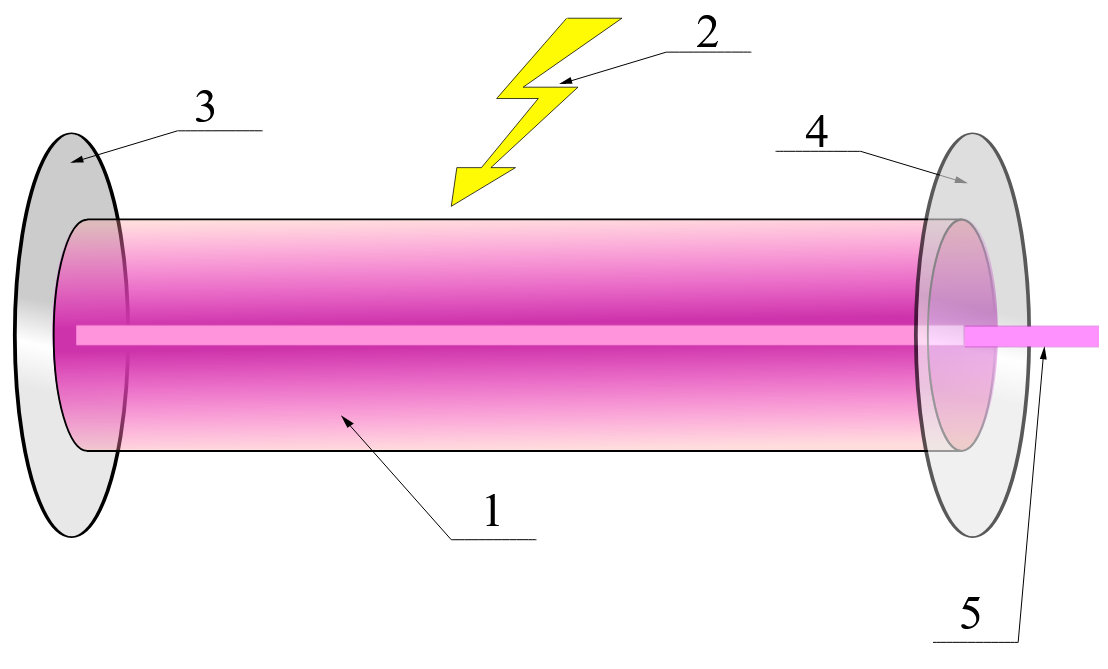
\includegraphics[width=0.4\textwidth]{Laser_Cavity.png}
        \vspace{-10pt}
        \caption{ 1. Gain medium , 2.Laser pumping energy, 3. High reflector , 4. Output coupler , 5. Laser Beam  \cite{Laser_cav} }
        
        \label{fig:lasercav}
    \end{wrapfigure}
    
    A laser operates by amplifying light through stimulated emission in a gain medium, fueled by an external energy source. 
    Optical feedback, often facilitated by mirrors within an optical cavity, promotes coherence. 
    Variations in laser design exist, but typically involve an output coupler and elements for beam manipulation. 
    These devices emit coherent light with controlled properties, akin to electronic oscillators. \\
    \subsubsection{Stimulated emission}
    Stimulated emission is a fundamental process in laser physics, characterized by the emission of a photon from an already excited atom when stimulated by the presence of a photon with frequency $\nu_{12}$ corresponding to the energy gap $\Delta E$ of the excited state to ground state transition. 
    Mathematically, the rate of stimulated emission is expressed as proportional to the number of atoms $N_2$ in the excited state and the radiation density of the light. 
    This relationship is encapsulated by the Einstein coefficients. 
    Specifically, the probability of a photon causing stimulated emission in a single excited atom is exactly equal to the probability of a photon being absorbed by an atom in the ground state. 
    This equality holds when the numbers of atoms in the ground and excited states are equal, resulting in a balanced rate of stimulated emission and absorption. \\
    For a laser to function effectively, the rate of stimulated emission must surpass that of absorption, necessitating a population inversion where $N_2$/$N_1$ > 1. 
    In other words, the population of the excited state must exceed that of the ground state. 
    %\begin{wrapfigure}[13]{l}[0cm]{0.3\textwidth}
    %    \centering
    %    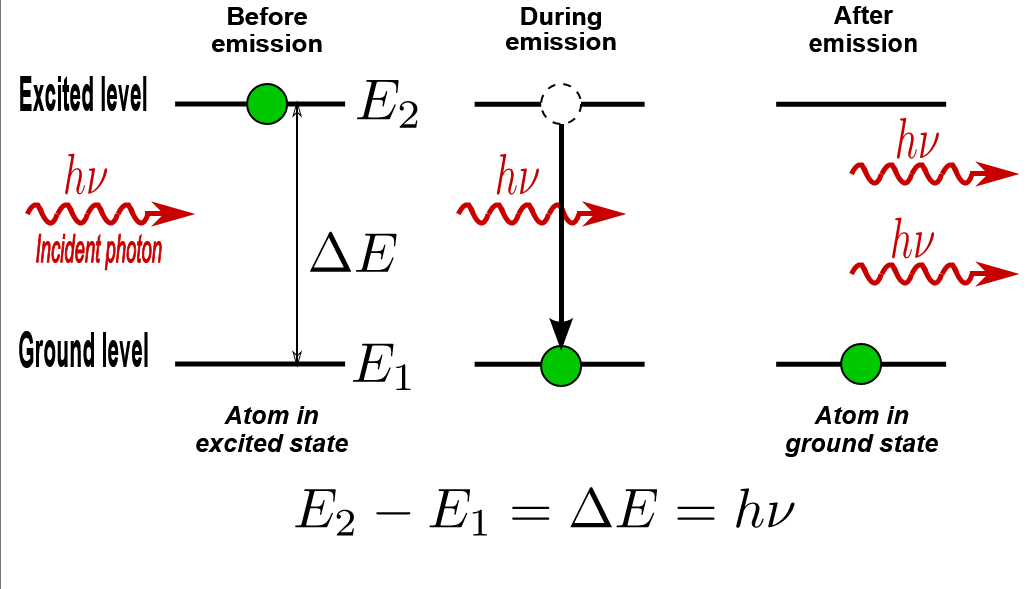
\includegraphics[width=0.3\textwidth]{Stim_Emission.png}
    %    
    %    \caption[width = 0.1\textwidth]{ Stimulated Emission  \cite{Laser_cav} }
    %    \label{fig:energy_diagram}
    %\end{wrapfigure}
    This condition allows for the production of a continuously increasing number of photons, establishing optical gain within the laser medium.
    Understanding the interplay between absorption, stimulated emission, and population inversion is crucial for the design and operation of laser systems. 
    By harnessing stimulated emission and achieving population inversion, lasers can amplify light coherently, enabling applications ranging from scientific research to industrial manufacturing.
    \monofig{width = 0.5\textwidth}{Stim_Emission.png}{ Stimulated Emission  \cite{Laser_cav} }{fig:energy_diagram}
\newpage
\subsection{Pulsed Lasers (Mode Locking)}
    % Describe pulsed lasers, their advantages, and limitations.
    % Discuss the concept of time-bandwidth limit and its relevance.
    Mode locking in optics is a technique used to generate ultra-short pulses of light in lasers, typically on the scale of picoseconds or femtoseconds. 
    By inducing a fixed phase relationship between the longitudinal modes of the laser's resonant cavity, constructive interference between these modes produces synchronized pulses. 
    This method, known as mode locking, alters the behavior of the laser's modes, causing them to periodically constructively interfere and emit intense bursts of light. 
    The pulse duration is determined by the number of locked modes and their frequency separation, governed by the laser's spectral width. 
    Mode locking enables precise control over pulse durations, with applications ranging from scientific research to industrial and medical fields.

\subsection{Second Harmonic Generation (SHG)}
    % Introduce SHG as a nonlinear optical process.
    % Explain how crystals generate light at twice the input frequency.
    % Discuss the importance of phase matching.
    Second-harmonic generation (SHG), or frequency doubling, is a fundamental nonlinear optical process where two photons with the same frequency interact in a nonlinear material, combining to generate a new photon with double the energy.
    This results in a photon with twice the frequency and half the wavelength of the initial photons,
    \begin{wrapfigure}[16]{r}[0cm]{0.4\textwidth}
        \centering
        \vspace{-\normalbaselineskip}
        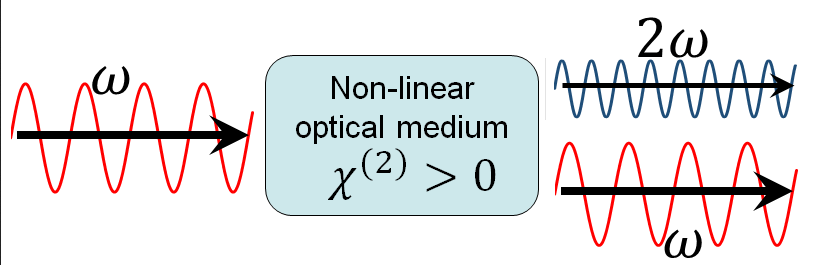
\includegraphics[width=0.4\textwidth]{shg_schem.png}
        \vspace{-10pt}
        \caption{Second harmonic generation }
        
        \label{fig:shg:basic}
    \end{wrapfigure}
    conserving excitation coherence. SHG is utilized extensively, particularly in doubling laser frequencies, and is governed by the second-order nonlinear susceptibility of the medium. 
    While SHG is typically prohibited in media with inversion symmetry, exceptions exist, such as in non-centrosymmetric crystals. 
    Achieving efficient SHG often requires intense pulsed laser beams passing through large crystals with precise alignment for phase matching.

\subsection{Iodine Absorption}
    % Cover the absorption properties of iodine, including rotation, vibration, and temperature dependence.
    % Explain natural linewidth and temperature broadening effects.

    Iodine exhibits distinct absorption spectra, primarily governed by its rotational and vibrational transitions. These transitions occur due to the interaction of electromagnetic radiation with the iodine molecules.

    Rotation transitions correspond to changes in the rotational energy levels of iodine molecules. These transitions typically occur in the microwave region of the electromagnetic spectrum. As the temperature increases, the population of molecules in higher rotational energy states also increases, leading to broader absorption lines due to the Doppler effect.
    
    Vibrational transitions, on the other hand, involve changes in the vibrational energy levels of iodine molecules. These transitions occur in the infrared region of the spectrum. The absorption lines corresponding to vibrational transitions are sharper compared to rotational transitions.
    
    The absorption spectrum of iodine also exhibits natural linewidth, which arises from the finite lifetime of excited states due to spontaneous emission. Additionally, temperature broadening effects broaden the absorption lines as the temperature of the sample increases, resulting in overlapping transitions and a continuous absorption spectrum.
    
    The absorbance $A$ of a sample can be calculated using the formula:
    
\begin{equation}
    A = -\log_{10}\left(\frac{I_t}{I_0}\right)
\end{equation}
    
    where 
    $I_0$ is the intensity of the incident light and
    $I_t$ is the intensity of the transmitted light through the sample.

\subsection{Grating Spectrometer}
    % Briefly mention grating spectrometers and their role in analyzing laser spectra.
    % Explain how diffraction gratings disperse light for spectral measurements.





\subsection{Uncertainty analysis}
\label{sec:unsichi}

In the entire protocol, unless otherwise specified, the maximum uncertainty method according to Eq.\ref{equ:groestunsicherheit} \cite{MMETH} is used for all error calculations.
For this purpose, the total differential of the outgoing equation is formed and the absolute values of the summands are multiplied by the uncertainty determined.
All statistical evaluations are subject to a statistical uncertainty according to the Student's t-distribution.
\begin{equation}
    \varDelta f = \biggl| \frac{\partial f}{\partial x_{1}} \cdot \varDelta x_{1} \biggl| + \biggl| \frac{\partial f}{\partial x_{2}} \cdot \varDelta x_{2} \biggl| + .... + \biggl| \frac{\partial f}{\partial x_{n}} \cdot \varDelta x_{n} \biggl|
    \label{equ:groestunsicherheit}
\end{equation}
\newpage